\documentclass[12pt]{article}
\newif\ifanswer\answertrue%\answerfalse% comment out to show/hide answers
\usepackage{../preamble}% preamble always after \newif\ifanswer
%\pagenumbering{gobble}
\title{Art Of Problem Solving - AMC 10 \\ Week 1}
\author{Patrick \& James Toche}
\date{June 11, 2021}

\begin{document}
\maketitle
\begin{minipage}{\textwidth}
\begin{abstract}\setlength{\parindent}{0pt}%
Homework for the AMC-10 Course by Art Of Problem Solving (AOPS).
Copyright restrictions may apply. Written for personal use. 
Please report typos and errors over at \url{https://github.com/ptoche/Math/tree/master/aops}. 
\end{abstract}
\end{minipage}

\thispagestyle{empty}
\clearpage


%%%%%%%%%%%%%%%%%%%%%%%%%%%%%%%%%%%%%%%%%%%%%%%%%%%%%%%%%%%%%%%%%%%%%%%%
\subsection*{1.}

\nopagebreak

The number of real values of $x$ that satisfy the equation
\begin{align*}
\left(2^{6x+3}\right) \left(4^{3x+6}\right) = 8^{4x+5}
\end{align*}
is:

\nopagebreak

\fbox{zero, $\quad$ one, $\quad$ two, $\quad$ three, $\quad$ greater than $3$}

\begin{answer}
We bring all exponentials to the same basis:
\begin{align*}
2^{6x+3} \cdot 2^{2(3x+6)} & = 2^{3(4x+5)} \\[1em]
            6x+3 + 2(3x+6) & = 3(4x+5) \\[1em]
                  12x + 15 & = 12x + 15
\end{align*}
which is always true. Thus, there are an infinity of solutions. And since $\infty>3$
\begin{empheq}[box={\mathbox[colback=white]}]{equation*}
    \text{The number of real values of $x$ is greater than $3$.}
\end{empheq} 
Note that we knew right away that the equation could be made linear by a change of the basis and that therefore the number of solutions had to be either $0$, $1$ or $\infty$, with $1$ the ``non-pathological'' case. So if we had been in a hurry, a good bet would have been $1$. Unfortunately, we would have lost the best in this case. 
\end{answer}
%%%%%%%%%%%%%%%%%%%%%%%%%%%%%%%%%%%%%%%%%%%%%%%%%%%%%%%%%%%%%%%%%%%%%%%%

\iftoggle{showAnswers}{\newpage}

%%%%%%%%%%%%%%%%%%%%%%%%%%%%%%%%%%%%%%%%%%%%%%%%%%%%%%%%%%%%%%%%%%%%%%%%
\subsection*{2.}

\nopagebreak

For which of the following values of $k$ does the equation
\begin{align*}
\frac{x-1}{x-2} = \frac{x-k}{x-6}
\end{align*}
have no solution for $x$?

\nopagebreak

\fbox{$k=1,\quad k=2,\quad k=3,\quad k=4,\quad k=5$}

\begin{answer}
We immediately note that the case $k=1$ is special. Substituting $k=1$ yields:
\begin{align*}
\frac{x-1}{x-2} = \frac{x-1}{x-6}
\end{align*}
At this point it is tempting to cancel out the $x-1$. But remember the question: when is there \textit{no} solution? Thus if we find one solution for some $k$, we can move on to the next value of $k$. We do not need to find all the solutions! And since $x=1$ is a solution of the above, we can rule out $k=1$. There are still four more cases to consider. 

We could go on substituting each possible value of $k$ and looking for solutions. Let's do it for one more case, as an exercise. Let $k=2$.
\begin{align*}
\frac{x-1}{x-2} & = \frac{x-2}{x-6} \\
     (x-1)(x-6) & = (x-2)^2 \\
   x^2 - 7x + 6 & = x^2 - 4x + 2 \\ 
             3x & = 4 \\
              x & = 4/3 
\end{align*}
Thus, there is a valid solution for $k=2$ (that solution is $x=4/3$). 

The other cases could be resolved with similar steps. But trying five cases will take a lot of work. So is there a quicker method? Let's be general:
\begin{align*}
\frac{x-1}{x-2} & = \frac{x-k}{x-6} \\
     (x-1)(x-6) & = (x-2)(x-k) \\
   x^2 - 7x + 6 & = x^2 - (2+k)x + 2k \\
       - 7x + 6 & = - (2+k)x + 2k
\end{align*}
Now note that if $7=2+k$, the $x$ term cancels out of the equation. And thus, there is no solution (the equation is impossible) if the following holds: 
\begin{align*}
         7 & = 2 + k \\
         6 & \neq 2k
\end{align*}
which is true for $k=5$. 

\begin{empheq}[box={\mathbox[colback=white]}]{equation*}
    k = 5
\end{empheq} 
\end{answer}
%%%%%%%%%%%%%%%%%%%%%%%%%%%%%%%%%%%%%%%%%%%%%%%%%%%%%%%%%%%%%%%%%%%%%%%%

\iftoggle{showAnswers}{\newpage}

%%%%%%%%%%%%%%%%%%%%%%%%%%%%%%%%%%%%%%%%%%%%%%%%%%%%%%%%%%%%%%%%%%%%%%%%
\subsection*{3.}

\nopagebreak

How many ordered triples $(a,b,c)$ of nonzero real numbers have the property that each number is the product of the other two?

\nopagebreak

\fbox{$1,\quad 2,\quad 3,\quad 4,\quad 5$}

\begin{answer}
We are looking for $(a,b,c)$, where $a\neq0$, $b\neq0$, $c\neq0$, such that:
\begin{align*}
a = bc \\
b = ac \\
c = ab
\end{align*}
We notice that this implies:
\begin{align*}
           abc & = 1 \\
\frac{abc}{bc} & = \frac{1}{a} \\
           a^2 & = 1 \\
             a & = \pm 1
\end{align*}
By symmetry, we also have $b=\pm1$, $c=\pm1$. So the candidate unordered-triples are $(1,1,1)$, $(1,1,-1)$, $(1,-1,-1)$, and $(-1,-1,-1)$. But clearly we need to be able to permute the symbols pairwise without violating the equality, which means only these are candidates: $(1,1,1)$ and $(1,-1,-1)$. That is triples. But the question asks for \textbf{ordered} triples. If the triple is ordered, $(+1,-1,-1)$, $(-1,+1,-1)$, and $(-1,-1,+1)$ are distinct. So altogether that gives $4$ ordered triples

\begin{empheq}[box={\mathbox[colback=white]}]{equation*}
    2 ~\text{non-ordered triples}, ~ 4 ~\text{ordered triples}
\end{empheq} 
\end{answer}
%%%%%%%%%%%%%%%%%%%%%%%%%%%%%%%%%%%%%%%%%%%%%%%%%%%%%%%%%%%%%%%%%%%%%%%%

\iftoggle{showAnswers}{\newpage}

%%%%%%%%%%%%%%%%%%%%%%%%%%%%%%%%%%%%%%%%%%%%%%%%%%%%%%%%%%%%%%%%%%%%%%%%
\subsection*{4.}

\nopagebreak

Two non-zero real numbers, $a$ and $b$, satisfy $ab = a - b$. Which of the following is a possible value of $\dfrac{a}{b} + \dfrac{b}{a} - ab$?

\nopagebreak

\fbox{$-2,\quad -1/2,\quad 1/3,\quad 1/2,\quad 2$}

\begin{answer}
Addition/subtraction is typically simpler than multiplication, so we are tempted to replace every instance of $ab$ with $a-b$ and hope that it will yield easy simplifications. We also see that if we bring the fractions to the same denominator, the product $ab$ will appear:
\begin{align*}
\frac{a}{b} + \frac{b}{a} = \frac{a^2 + b^2}{ab}
\end{align*}
The appearance of $a^2 + b^2$ is not very encouraging. However since we know something about $a-b$, we are reminded that $(a-b)^2$ generates $a^2 + b^2$. So we take it from here:
\begin{align*}
       (a-b)^2 & = a^2 + b^2 -2ab \\
     a^2 + b^2 & = (a-b)^2 + 2ab \\
     a^2 + b^2 & = (ab)^2 + 2ab 
\end{align*}
Substituting back in:
\begin{align*}
\frac{a}{b} + \frac{b}{a} & = \frac{a^2 + b^2}{ab} \\
                          & = \frac{(ab)^2 + 2ab}{ab} \\
                          & = ab + 2
\end{align*}
And thus
\begin{empheq}[box={\mathbox[colback=white]}]{equation*}
    \frac{a}{b} + \frac{b}{a} - ab = 2
\end{empheq} 
\end{answer}
%%%%%%%%%%%%%%%%%%%%%%%%%%%%%%%%%%%%%%%%%%%%%%%%%%%%%%%%%%%%%%%%%%%%%%%%

\iftoggle{showAnswers}{\newpage}

%%%%%%%%%%%%%%%%%%%%%%%%%%%%%%%%%%%%%%%%%%%%%%%%%%%%%%%%%%%%%%%%%%%%%%%%
\subsection*{5.}

\nopagebreak

If $a + 1 = b + 2 = c + 3 = d + 4 = a + b + c + d + 5$, then $a + b + c + d$ is

\nopagebreak

\fbox{$-5,\quad -10/3,\quad -7/3,\quad 5/3,\quad 5$}

\begin{answer}
It pays to rewrite these for clarity:
\begin{align*}
a + 1 & = b + 2 \\
b + 2 & = c + 3 \\
c + 3 & = d + 4\\
d + 4 & = a + b + c + d + 5
\end{align*}
This shows that we have $4$ linear equations in $4$ unknowns, which we expect to be able to solve. But can we get the sum faster than that? If we add up the equations or multiply them, we get a lot of cancellations, but the answer does not come out right away. Let's introduce new variables to see the pattern:
\begin{align*}
     s & = a + b + c + d \\
\alpha & = a + 1\\ 
 \beta & = b + 2\\ 
\gamma & = c + 3\\ 
\delta & = d + 4 
\end{align*}
We want to find $s = \delta -5$, where
\begin{align*}
\alpha & = \beta \\
 \beta & = \gamma \\
\gamma & = \delta \\
\delta & = \alpha + \beta + \gamma + \delta - 5
\end{align*}
where the last equation comes from:
\begin{center}
\newcolumntype{z}{>{$}c<{$}}%
\begin{tabular}{@{}zzzzzzzzzzz@{}}
\delta & = &      a & + &     b & + &      c & + &      d & + & 5 \\[1ex]
       & = &  (a+1) & + & (b+2) & + &  (c+3) & + &  (d+4) & + & 5-1-2-3-4 \\[1ex]
       & = & \alpha & + & \beta & + & \gamma & + & \delta & - & 5 \\
\end{tabular}
\end{center}
Now we have a reasonably simple way to get the answer. Since $\alpha$ $=$ $\beta$ $=$ $\gamma$ $=$ $\delta$,
\begin{align*}
\delta & = \alpha + \beta + \gamma + \delta - 5 \\
\delta & = \delta + \delta + \delta + \delta - 5 \\
                 \delta & = 5/3 \\[1ex]
\Rightarrow \quad
                      s & = 5/3 -5 = -10/3
\end{align*}

\begin{empheq}[box={\mathbox[colback=white]}]{equation*}
    a + b + c + d = \frac{-10}{3}
\end{empheq} 
\end{answer}
%%%%%%%%%%%%%%%%%%%%%%%%%%%%%%%%%%%%%%%%%%%%%%%%%%%%%%%%%%%%%%%%%%%%%%%%

\iftoggle{showAnswers}{\newpage}

%%%%%%%%%%%%%%%%%%%%%%%%%%%%%%%%%%%%%%%%%%%%%%%%%%%%%%%%%%%%%%%%%%%%%%%%
\subsection*{6.}

\nopagebreak

Let $a$, $b$, $c$, and $d$ be real numbers with $|a - b| = 2$, $|b - c| = 3$, and $|c - d| = 4$. What is the sum of all possible values of $|a - d|$?

\nopagebreak

\fbox{$9,\quad 12,\quad 15,\quad 18,\quad 24$}

\begin{answer}
The problem is to solve for $x = |a - d|$, where:
\begin{align*}
|a - b| & = 2 \\
|b - c| & = 3 \\
|c - d| & = 4
\end{align*}
We have several cases to consider:
\begin{align*}
& 
\begin{cases}
a - b = 2 \\
a - b = -2 
\end{cases}\\
& 
\begin{cases}
b - c = 3 \\
b - c = -3
\end{cases}\\
& 
\begin{cases}
c - d = 4 \\
c - d = -4
\end{cases}
\end{align*}
We can get $a-d$ by adding the three cases. For instance:
\begin{align*}
a - b & = 2 \\
b - c & = 3 \\
c - d & = 4 \\[1em]
a - d & = 2 + 3 + 4 = 9
\end{align*}
So now we repeat the pattern for all possible values of $a-d$:
\begin{align*}
a - d & = +2 + 3 + 4 = +9 \\
      & = -2 + 3 + 4 = +5 \\
      & = +2 - 3 + 4 = +3 \\
      & = +2 + 3 - 4 = +1 \\
      & = -2 - 3 + 4 = -1 \\
      & = -2 + 3 - 4 = -3 \\
      & = +2 - 3 - 4 = -5 \\
      & = -2 - 3 - 4 = -9 
\end{align*}
But we are looking for $|a-d|$, so adding up the positive values gives:

\begin{align*}
|a - d| = 1 + 3 + 5 + 9 = 18
\end{align*}

\begin{empheq}[box={\mathbox[colback=white]}]{equation*}
    |a - d| = 18
\end{empheq} 
\end{answer}
%%%%%%%%%%%%%%%%%%%%%%%%%%%%%%%%%%%%%%%%%%%%%%%%%%%%%%%%%%%%%%%%%%%%%%%%

\iftoggle{showAnswers}{\newpage}

%%%%%%%%%%%%%%%%%%%%%%%%%%%%%%%%%%%%%%%%%%%%%%%%%%%%%%%%%%%%%%%%%%%%%%%%
\subsection*{7.}

\nopagebreak

If $x$ and $y$ are nonzero numbers such that $x = 1 + \frac{1}{y}$ and $y = 1 + \frac{1}{x}$, then $y$ equals

\nopagebreak

\fbox{$x-1,\quad 1-x,\quad 1+x,\quad -x,\quad x$}

\begin{answer}
\begin{align*}
x & = 1 + \frac{1}{y} \\
y & = 1 + \frac{1}{x}
\end{align*}
The symmetry of the problem is obvious and indeed:
\begin{align*}
xy & = y + 1 \\
yx & = x + 1 \\
\Rightarrow \quad x & = y \qquad\qed
\end{align*}

\begin{empheq}[box={\mathbox[colback=white]}]{equation*}
    y = x
\end{empheq} 

Out of curiosity, let's solve the quadratic equation:
\begin{align*}
x & = 1 + \frac{1}{x} \\
x^2 - x - 1 & = 0\\
   \left(x - \frac{1}{2}\right)^2 - \left(\frac{1}{2}\right)^2 - 1 & = 0 \\ 
\left(x - \frac{1}{2}\right)^2 - \left(\frac{\sqrt{5}}{2}\right)^2 & = 0 \\
(x - \frac{1+\sqrt{5}}{2}) (x - \frac{1-\sqrt{5}}{2}) & = 0  \\
    y = \frac{1+\sqrt{5}}{2}, \frac{1-\sqrt{5}}{2}
\end{align*}
\end{answer}
%%%%%%%%%%%%%%%%%%%%%%%%%%%%%%%%%%%%%%%%%%%%%%%%%%%%%%%%%%%%%%%%%%%%%%%%

\iftoggle{showAnswers}{\newpage}

%%%%%%%%%%%%%%%%%%%%%%%%%%%%%%%%%%%%%%%%%%%%%%%%%%%%%%%%%%%%%%%%%%%%%%%%
\subsection*{8.}

\nopagebreak

A right triangle has perimeter 32 and area 20. What is the length of its hypotenuse?

\nopagebreak

\fbox{$\dfrac{57}{4},\quad \dfrac{59}{4},\quad \dfrac{61}{4},\quad \dfrac{63}{4},\quad \dfrac{65}{4}$}

\begin{answer}
Let $a$, $b$ denote the lengths of the legs and $c$ the length of the hypotenuse. 

\begin{center}
  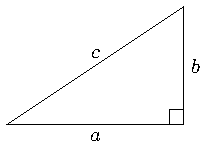
\includegraphics[height=3cm,page=1]{2021-06-11-figure-08}
\end{center}

We know these facts:
\begin{alignat*}{3}
\text{area:}\quad      && \frac{ab}{2} && \quad=\quad 20\\
\text{perimeter:}\quad &&    a + b + c && \quad=\quad 32 
\end{alignat*}
We want to solve for $c$, which is related to $a$ and $b$ by the Pythagorean triangle identity:
\begin{align*}
c & = \sqrt{a^2+b^2}
\end{align*}
To get an expression involving $a^2$ and $b^2$ , we square the perimeter formula:
\begin{align*}
          a + b & = 32 -c \\
      (a + b)^2 & = (32 -c)^2 \\
a^2 + b^2 + 2ab & = 32^2 - 64 c + c^2 \\
       c^2 + 80 & = 1024 - 64 c + c^2 \\
            64c & = 944 \\
              c & = \frac{944}{64} 
                  = \frac{59}{4}
\end{align*}

\begin{empheq}[box={\mathbox[colback=white]}]{equation*}
    \text{length of hypotenuse:}~\frac{59}{4}
\end{empheq} 
\end{answer}
%%%%%%%%%%%%%%%%%%%%%%%%%%%%%%%%%%%%%%%%%%%%%%%%%%%%%%%%%%%%%%%%%%%%%%%%

\iftoggle{showAnswers}{\newpage}

%%%%%%%%%%%%%%%%%%%%%%%%%%%%%%%%%%%%%%%%%%%%%%%%%%%%%%%%%%%%%%%%%%%%%%%%
\subsection*{9.}

\nopagebreak

Let $a$, $b$, $c$ be real numbers such that $a - 7b + 8c = 4$ and $8a + 4b - c = 7$. Then $a^2 - b^2 + c^2$ is

\nopagebreak

\fbox{$0,\quad 1,\quad 4,\quad 7,\quad 8$}

\begin{answer}
We have a linear system of two equations in three unknowns $a$, $b$, $c$:
\begin{align*}
a - 7b + 8c & = 4 \\ 
8a + 4b - c & = 7
\end{align*}
We notice a $1,4,7,8$ pattern. The key insight is that the first equation has $(1a,8c)$ and the second $(8a,-1c)$, while $b$ appears with different coefficients. This suggests squaring both equations after a clever rearrangement:
\begin{align*}
\left(a + 8c\right)^2 & = \left(4 + 7b\right)^2  \\ 
\left(8a - c\right)^2 & = \left(7 - 4b\right)^2 
\end{align*}
Distributing:
\begin{align*}
  a^2 + 16ac + 64c^2 & = 16 + 56b + 49b^2  \\ 
64a^2 - 16ac +   c^2 & = 49 - 56b + 16b^2
\end{align*}
Adding up:
\begin{align*}
65a^2 + 65 c^2 & = 65 + 65b^2 \\
\Rightarrow \quad
a^2 - b^2 + c^2 & = 1
\end{align*}

\begin{empheq}[box={\mathbox[colback=white]}]{equation*}
    a^2 - b^2 + c^2 = 1
\end{empheq} 
\end{answer}
%%%%%%%%%%%%%%%%%%%%%%%%%%%%%%%%%%%%%%%%%%%%%%%%%%%%%%%%%%%%%%%%%%%%%%%%

\iftoggle{showAnswers}{\newpage}

%%%%%%%%%%%%%%%%%%%%%%%%%%%%%%%%%%%%%%%%%%%%%%%%%%%%%%%%%%%%%%%%%%%%%%%%
\subsection*{10.}

\nopagebreak

Suppose that the number $a$ satisfies the equation $4 = a + a^{-1}$. What is the value of $a^4 + a^{-4}$?

\nopagebreak

\fbox{$164,\quad 172,\quad 192,\quad 194,\quad 212$}

\begin{answer}
Let's expand the binomial. The coefficients of Pascal's triangle are $1$, $4$, $6$, $4$, $1$.
\begin{align*}
\left(a + a^{-1}\right)^4 
  & =     a^4 \cdot \left(a^{-1}\right)^0 
    + 4 a^{3} \cdot \left(a^{-1}\right)^1 
    + 6 a^{2} \cdot \left(a^{-1}\right)^2 
    + 4 a^{1} \cdot \left(a^{-1}\right)^3 
    +   a^{0} \cdot \left(a^{-1}\right)^4 \\
  & = a^4 + 4 a^{2} + 6 + 4 a^{-2} + a^{-4} \\
  & = a^4 +  a^{-4} + 6 + 4 (a^{2} + a^{-2})
\end{align*}
Rearranging and setting $(a+a^{-1})^4=4^4$,
\begin{align*}
a^4 +  a^{-4}
  & = 4^4 - 6 - 4 (a^{2} + a^{-2})
\end{align*}
Expanding the binomial again:
\begin{align*}
\left(a + a^{-1}\right)^2 
  & =     a^2 \cdot \left(a^{-1}\right)^0 
    + 2 a^{1} \cdot \left(a^{-1}\right)^1 
    +   a^{0} \cdot \left(a^{-1}\right)^2 \\
  & = a^2 + 2 + a^{-2}
\end{align*}
Rearranging and setting $(a+a^{-1})^2=4^2$,
\begin{align*}
a^2 + a^{-2} = 4^2 - 2 = 14
\end{align*}
Plugging this back into the previous expression:
\begin{align*}
a^4 +  a^{-4}
  & = 4^4 - 6 - 4 \cdot 14 \\
  & = 194
\end{align*}
\begin{empheq}[box={\mathbox[colback=white]}]{equation*}
    a^4 +  a^{-4} = 194
\end{empheq} 
\end{answer}
%%%%%%%%%%%%%%%%%%%%%%%%%%%%%%%%%%%%%%%%%%%%%%%%%%%%%%%%%%%%%%%%%%%%%%%%

\end{document}
